\tikzset{every picture/.style={line width=0.75pt}} %set default line width to 0.75pt        

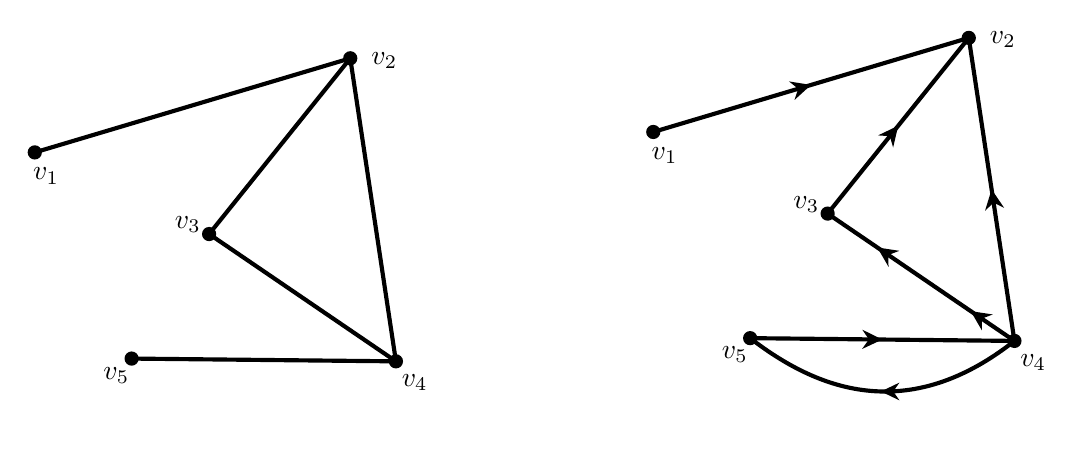
\begin{tikzpicture}[x=0.5pt,y=0.5pt,yscale=-1,xscale=1]
%uncomment if require: \path (0,306); %set diagram left start at 0, and has height of 306

%Flowchart: Connector [id:dp6790201336903005] 
\draw  [fill={rgb, 255:red, 0; green, 0; blue, 0 }  ,fill opacity=1 ] (89,103) .. controls (89,100.58) and (90.96,98.62) .. (93.38,98.62) .. controls (95.79,98.62) and (97.75,100.58) .. (97.75,103) .. controls (97.75,105.42) and (95.79,107.38) .. (93.38,107.38) .. controls (90.96,107.38) and (89,105.42) .. (89,103) -- cycle ;
%Flowchart: Connector [id:dp8323400540036575] 
\draw  [fill={rgb, 255:red, 0; green, 0; blue, 0 }  ,fill opacity=1 ] (317,35) .. controls (317,32.58) and (318.96,30.62) .. (321.38,30.62) .. controls (323.79,30.62) and (325.75,32.58) .. (325.75,35) .. controls (325.75,37.42) and (323.79,39.38) .. (321.38,39.38) .. controls (318.96,39.38) and (317,37.42) .. (317,35) -- cycle ;
%Flowchart: Connector [id:dp4253552390250358] 
\draw  [fill={rgb, 255:red, 0; green, 0; blue, 0 }  ,fill opacity=1 ] (350,254) .. controls (350,251.58) and (351.96,249.62) .. (354.38,249.62) .. controls (356.79,249.62) and (358.75,251.58) .. (358.75,254) .. controls (358.75,256.42) and (356.79,258.38) .. (354.38,258.38) .. controls (351.96,258.38) and (350,256.42) .. (350,254) -- cycle ;
%Flowchart: Connector [id:dp15161486550981407] 
\draw  [fill={rgb, 255:red, 0; green, 0; blue, 0 }  ,fill opacity=1 ] (159,252) .. controls (159,249.58) and (160.96,247.62) .. (163.38,247.62) .. controls (165.79,247.62) and (167.75,249.58) .. (167.75,252) .. controls (167.75,254.42) and (165.79,256.38) .. (163.38,256.38) .. controls (160.96,256.38) and (159,254.42) .. (159,252) -- cycle ;
%Straight Lines [id:da33485918253219815] 
\draw [color={rgb, 255:red, 0; green, 0; blue, 0 }  ,draw opacity=1 ][line width=1.5]    (93.38,103) -- (321.38,35) ;
%Flowchart: Connector [id:dp6607903165665847] 
\draw  [fill={rgb, 255:red, 0; green, 0; blue, 0 }  ,fill opacity=1 ] (215,162) .. controls (215,159.58) and (216.96,157.62) .. (219.38,157.62) .. controls (221.79,157.62) and (223.75,159.58) .. (223.75,162) .. controls (223.75,164.42) and (221.79,166.38) .. (219.38,166.38) .. controls (216.96,166.38) and (215,164.42) .. (215,162) -- cycle ;
%Straight Lines [id:da9704902392723933] 
\draw [color={rgb, 255:red, 0; green, 0; blue, 0 }  ,draw opacity=1 ][line width=1.5]    (219.38,162) -- (321.38,35) ;
%Straight Lines [id:da3214089668075706] 
\draw [color={rgb, 255:red, 0; green, 0; blue, 0 }  ,draw opacity=1 ][line width=1.5]    (163.38,252) -- (354.38,254) ;
%Straight Lines [id:da35660925127636145] 
\draw [color={rgb, 255:red, 0; green, 0; blue, 0 }  ,draw opacity=1 ][line width=1.5]    (354.38,254) -- (321.38,35) ;
%Straight Lines [id:da32904194418935273] 
\draw [color={rgb, 255:red, 0; green, 0; blue, 0 }  ,draw opacity=1 ][line width=1.5]    (354.38,254) -- (219.38,162) ;
%Flowchart: Connector [id:dp12548501893331887] 
\draw  [fill={rgb, 255:red, 0; green, 0; blue, 0 }  ,fill opacity=1 ] (536,88.24) .. controls (536,85.82) and (537.96,83.86) .. (540.38,83.86) .. controls (542.79,83.86) and (544.75,85.82) .. (544.75,88.24) .. controls (544.75,90.65) and (542.79,92.61) .. (540.38,92.61) .. controls (537.96,92.61) and (536,90.65) .. (536,88.24) -- cycle ;
%Flowchart: Connector [id:dp6716572124529165] 
\draw  [fill={rgb, 255:red, 0; green, 0; blue, 0 }  ,fill opacity=1 ] (764,20.24) .. controls (764,17.82) and (765.96,15.86) .. (768.38,15.86) .. controls (770.79,15.86) and (772.75,17.82) .. (772.75,20.24) .. controls (772.75,22.65) and (770.79,24.61) .. (768.38,24.61) .. controls (765.96,24.61) and (764,22.65) .. (764,20.24) -- cycle ;
%Flowchart: Connector [id:dp08043752132546567] 
\draw  [fill={rgb, 255:red, 0; green, 0; blue, 0 }  ,fill opacity=1 ] (797,239.24) .. controls (797,236.82) and (798.96,234.86) .. (801.38,234.86) .. controls (803.79,234.86) and (805.75,236.82) .. (805.75,239.24) .. controls (805.75,241.65) and (803.79,243.61) .. (801.38,243.61) .. controls (798.96,243.61) and (797,241.65) .. (797,239.24) -- cycle ;
%Flowchart: Connector [id:dp2016204031515907] 
\draw  [fill={rgb, 255:red, 0; green, 0; blue, 0 }  ,fill opacity=1 ] (606,237.24) .. controls (606,234.82) and (607.96,232.86) .. (610.38,232.86) .. controls (612.79,232.86) and (614.75,234.82) .. (614.75,237.24) .. controls (614.75,239.65) and (612.79,241.61) .. (610.38,241.61) .. controls (607.96,241.61) and (606,239.65) .. (606,237.24) -- cycle ;
%Straight Lines [id:da9124210665741758] 
\draw [color={rgb, 255:red, 0; green, 0; blue, 0 }  ,draw opacity=1 ][line width=1.5]    (540.38,88.24) -- (768.38,20.24) ;
\draw [shift={(654.38,54.24)}, rotate = 163.39] [fill={rgb, 255:red, 0; green, 0; blue, 0 }  ,fill opacity=1 ][line width=0.08]  [draw opacity=0] (14.56,-6.99) -- (0,0) -- (14.56,6.99) -- (9.67,0) -- cycle    ;
%Flowchart: Connector [id:dp17378293402374523] 
\draw  [fill={rgb, 255:red, 0; green, 0; blue, 0 }  ,fill opacity=1 ] (662,147.24) .. controls (662,144.82) and (663.96,142.86) .. (666.38,142.86) .. controls (668.79,142.86) and (670.75,144.82) .. (670.75,147.24) .. controls (670.75,149.65) and (668.79,151.61) .. (666.38,151.61) .. controls (663.96,151.61) and (662,149.65) .. (662,147.24) -- cycle ;
%Straight Lines [id:da42496408917755524] 
\draw [color={rgb, 255:red, 0; green, 0; blue, 0 }  ,draw opacity=1 ][line width=1.5]    (666.38,147.24) -- (768.38,20.24) ;
\draw [shift={(717.38,83.74)}, rotate = 128.77] [fill={rgb, 255:red, 0; green, 0; blue, 0 }  ,fill opacity=1 ][line width=0.08]  [draw opacity=0] (14.56,-6.99) -- (0,0) -- (14.56,6.99) -- (9.67,0) -- cycle    ;
%Straight Lines [id:da352612778908305] 
\draw [color={rgb, 255:red, 0; green, 0; blue, 0 }  ,draw opacity=1 ][line width=1.5]    (610.38,237.24) -- (801.38,239.24) ;
\draw [shift={(705.88,238.24)}, rotate = 180.6] [fill={rgb, 255:red, 0; green, 0; blue, 0 }  ,fill opacity=1 ][line width=0.08]  [draw opacity=0] (14.56,-6.99) -- (0,0) -- (14.56,6.99) -- (9.67,0) -- cycle    ;
%Straight Lines [id:da014195829977063146] 
\draw [color={rgb, 255:red, 0; green, 0; blue, 0 }  ,draw opacity=1 ][line width=1.5]    (801.38,239.24) -- (768.38,20.24) ;
\draw [shift={(784.88,129.74)}, rotate = 81.43] [fill={rgb, 255:red, 0; green, 0; blue, 0 }  ,fill opacity=1 ][line width=0.08]  [draw opacity=0] (14.56,-6.99) -- (0,0) -- (14.56,6.99) -- (9.67,0) -- cycle    ;
%Straight Lines [id:da2717088403944091] 
\draw [color={rgb, 255:red, 0; green, 0; blue, 0 }  ,draw opacity=1 ][line width=1.5]    (801.38,239.24) -- (738.18,196.17) -- (666.38,147.24) ;
\draw [shift={(769.78,217.7)}, rotate = 34.27] [fill={rgb, 255:red, 0; green, 0; blue, 0 }  ,fill opacity=1 ][line width=0.08]  [draw opacity=0] (14.56,-6.99) -- (0,0) -- (14.56,6.99) -- (9.67,0) -- cycle    ;
\draw [shift={(702.28,171.7)}, rotate = 34.27] [fill={rgb, 255:red, 0; green, 0; blue, 0 }  ,fill opacity=1 ][line width=0.08]  [draw opacity=0] (14.56,-6.99) -- (0,0) -- (14.56,6.99) -- (9.67,0) -- cycle    ;
%Curve Lines [id:da5145213870577791] 
\draw [line width=1.5]    (801.38,239.24) .. controls (719.63,303.76) and (652.63,269.76) .. (610.38,237.24) ;
\draw [shift={(704.9,275.77)}, rotate = 0.02] [fill={rgb, 255:red, 0; green, 0; blue, 0 }  ][line width=0.08]  [draw opacity=0] (13.4,-6.43) -- (0,0) -- (13.4,6.44) -- (8.9,0) -- cycle    ;

% Text Node
\draw (90,112) node [anchor=north west][inner sep=0.75pt]   [align=left] {$\displaystyle v_{1}$};
% Text Node
\draw (192.38,147.38) node [anchor=north west][inner sep=0.75pt]   [align=left] {$\displaystyle v_{3}$};
% Text Node
\draw (140.75,256) node [anchor=north west][inner sep=0.75pt]   [align=left] {$\displaystyle v_{5}$};
% Text Node
\draw (356.38,261.38) node [anchor=north west][inner sep=0.75pt]   [align=left] {$\displaystyle v_{4}$};
% Text Node
\draw (334.38,28.38) node [anchor=north west][inner sep=0.75pt]   [align=left] {$\displaystyle v_{2}$};
% Text Node
\draw (537,97.24) node [anchor=north west][inner sep=0.75pt]   [align=left] {$\displaystyle v_{1}$};
% Text Node
\draw (639.38,132.61) node [anchor=north west][inner sep=0.75pt]   [align=left] {$\displaystyle v_{3}$};
% Text Node
\draw (587.75,241.24) node [anchor=north west][inner sep=0.75pt]   [align=left] {$\displaystyle v_{5}$};
% Text Node
\draw (803.38,246.61) node [anchor=north west][inner sep=0.75pt]   [align=left] {$\displaystyle v_{4}$};
% Text Node
\draw (781.38,13.61) node [anchor=north west][inner sep=0.75pt]   [align=left] {$\displaystyle v_{2}$};


\end{tikzpicture}
